\chapter{The Standard Model}\label{ch:sm}
In this chapter we will describe the components of the Standard Model of particle physics, with particular attention to the theory of weak interactions. The treatment is semi-historical. We assume familiarity with the basic concepts of quantum field theory, including what a particle is, the connection between particles and fields, and basic group theory concepts. For a refresher, one may turn to \autoref{ch:qft}. We will first talk about the matter content, followed by a discussion of gauge invariance and how it leads to gauge fields that both interact with themselves and mediate the interactions between the matter fields. We will then briefly comment on the concept of renormalization in the context of the Standard Model, and finally conclude with highlighting the limits of the Standard Model and the need for new physics extensions to it. The material in this chapter draws from a number of excellent treatments of the subject \citep{Cheng1985,Schwartz2014,Zee2010,Peskin:1995ev}.

\section{Particle content}
The fundamental constituents of matter are fermions. They come in two varieties - quarks and leptons. Quarks are found in places such as atomic nuclei and in cosmic ray mesons. The most well-known example of leptons are electrons, that orbit atomic nuclei, but there are many other flavors of leptons as well. The full lists of quarks and leptons in the SM can be found in tables \ref{tab:quarks} and \ref{tab:leptons}. The particles that mediate the interactions between these are called \emph{gauge bosons}, and are listed in table \ref{tab:gaugebosons}. The photon is the mediator of the electromagnetic force, the $W$ and $Z$ bosons mediate the weak force, which is responsible for radioactive decay, and gluons mediate the strong force between quarks, which is responsible for the formation of protons, neutrons and other heavy particles.

\begin{margintable}[-10cm]
  \centering
  \begin{tabular}{c|l}
    Symbol & Name \\
  \hline
    $u$ & up\\
    $d$ & down \\
    $c$ & charm \\
    $s$ & strange \\
    $t$ & top \\
    $b$ & bottom \\
  \end{tabular}
  \caption{List of quarks in the SM.}
  \label{tab:quarks}
\end{margintable}

\begin{margintable}[-3cm]
  \centering
\begin{tabular}{c|l}
    Symbol & Name \\
  \hline
    $e$ & electron\\
    $\mu$ & muon \\
    $\tau$ & tau \\
    $\nu_e$ & top \\
    $\nu_\mu$ & bottom \\
    $\nu_\tau$ & bottom \\
  \end{tabular}
  \caption{List of leptons in the SM.}
  \label{tab:leptons}
\end{margintable}

\begin{margintable}
  \centering
\begin{tabular}{c|l}
    Symbol & Name \\
  \hline
    $\gamma$ & photon\\
    $W$ & $W$ boson \\
    $Z$ & $Z$ boson \\
    $g$ & gluon \\
  \end{tabular}
  \caption{List of gauge bosons in the SM.}
  \label{tab:gaugebosons}
\end{margintable}

The standard model Lagrangian can be split up as follows:

$$\L_{SM} = \L_{fermion}+\L_{gauge}+\L_{Higgs}.$$
In the absence of interactions, the Lagrangian for a free Dirac fermion field $\psi$ would read as follows\footnote{Here we emply the Feynman slash notation, with $\gamma^\mu p_\mu = \slashed{p}$}.
\begin{align}
\L_{fermion} = i\overline{\psi}\slashed{\partial}_\mu\psi-m_{\psi}\overline{\psi}\psi.
\label{eq:fermion_lagrangian}
\end{align}

Interactions and the corresponding gauge bosons arise organically when we impose gauge invariance upon this Lagrangian.

\section{Gauge invariance}\label{sec:gauge_invariance}

The concept of gauge invariance arose in the context of electrodynamics, with the realization that there was an intrinsic degree of freedom for the electromagnetic vector potential $A_\mu$. Basically, under the transformation 
\begin{align}
  A_\mu\rightarrow A_\mu + \partial_\mu \lambda(x),
  \label{eq:gauge_transformation}
\end{align}
where $\lambda(x)$ is an arbitrary scalar function, the electromagnetic Lagrangian (and by extension, the Maxwell equations) remain invariant. In quantum mechanics (with an electromagnetic potential), the requirement that physical observables are not to change under gauge transformations is ensured by the simultaneous transformation of the state ket $|\psi\rangle\rightarrow e^{i\theta(x)}|\psi\rangle$ \citep{Sakurai2010}. The modern interpretation of gauge invariance %
%
\footnote{The origin of the term `gauge invariance' lies in Hermann Weyl's attempt to describe electromagnetism as a geometric theory, similar to gravity, in 1916. He hoped to recover electromagnetism by imposing an invariance, termed \emph{eichinvarianz} (which translates to gauge invariance in English)  under local scale transformations, and identifying the scale factor with the electromagnetic vector potential $A_\mu$. Although this attempt was unsuccessful, the term was retained when it was discovered the correct way forward was to impose invariance under \emph{phase} transformations instead of scale transformations. For a history of the origins of gauge invariance, see \citep{Jackson2001}.}%
%
is a geometric one, usually discussed among mathematicians in terms of fiber bundles and connections \citep{Cheng1985}. Although a full geometric treatment of this topic is beyond the scope of this work, a small digression into it is worthwhile.

In this section, we will attempt to heuristically construct the Lagrangian for quantum electrodynamics, using gauge invariance. Consider the Lagrangian for the free fermion field in \autoref{eq:fermion_lagrangian}. This remains invariant under the transformation 
\begin{equation}\label{eq:fermion_field_transformation}
  \psi(x)\rightarrow e^{i\theta(x)}\psi(x).
\end{equation}
Thus, the phase of a quantum field is an unobservable quantity. However, we often have to compare the values of fields at different points in spacetime - for example when we take the partial derivative $\partial_\mu$ in \autoref{eq:fermion_lagrangian}. At a very basic level, a derivative of a function $f(x)$ depends on the difference of the values of the function $f$ at the points $x$ and $x + dx$. However, the phase of the field is a matter of arbitrary convention, and our physical observables should not depend on them. To be able to compare fields at $x$ and $dx$, we need to promote our ordinary derivative $\partial_\mu$ to a \emph{gauge-covariant} or simply \emph{covariant} derivative,
$$\partial_\mu \rightarrow D_\mu = \partial_\mu - igA_\mu$$
Here, $A_\mu$ is a vector field that transforms as%
%
$$A_\mu\rightarrow A_\mu + \frac{1}{g}\partial_\mu\theta(x)$$
%
where $\lambda(x)$ is a scalar function and $g$ is a dimensionless constant, whose physical interpretation will soon become apparent. The covariant derivative is a mathematical concept that arises in the theory of general relativity as well, and the field $A_\mu$ can be identified with a \emph{connection}, which gives us a way to compare the fields at the points $x$ and $x + dx$.

Inserting the covariant derivative in the place of the normal partial derivative in equation in the kinetic term of \autoref{eq:fermion_lagrangian} gives us the following:
\begin{equation}\label{eq:fermion_kinetic}
    \begin{split}
  \mathcal{L}_\text{fermion, kinetic} &= i\overline{\psi}\slashed{D}_\mu\psi\\
&= i\overline{\psi}\gamma^\mu(\partial_\mu-igA_\mu)\psi\\
&= i\overline{\psi}\slashed{\partial}_\mu\psi + g\overline{\psi}A_\mu\psi
\end{split}
\end{equation}
The second term on the right hand side of \autoref{eq:fermion_kinetic} is the interaction term describing the interaction between the electromagnetic field and a fermion field. We can now identify $g$ with the coupling of $A_\mu$ to fermions, that is, the strength of the interaction.  However, we are not done yet. We know that for $A_\mu$ to mediate interactions, it must be a dynamical, or propagating field. This means that the Lagrangian must have a term involving its derivatives - this will serve as the kinetic term for $A_\mu$. The simplest such gauge-invariant term with dimension four or less is %
%
\begin{equation}\label{eq:L_gauge_kin}
\mathcal{L}_\text{gauge, kinetic} = -\frac{1}{4}F_{\mu\nu}F^{\mu\nu}
\end{equation}
%
where $F_{\mu\nu} = \partial_\mu A_\nu - \partial_\nu A_\mu$, and the factor $\slantfrac{1}{4}$ is just a convenient normalization convention. The astute reader will notice that this has begun to look suspiciously like the Lagrangian density for the classical electromagnetic field. In fact, the function $\frac{1}{g} \theta(x)$ can be identified with the function $\lambda(x)$ in \autoref{eq:gauge_transformation}, and the constant $g$ can be identified with the electric charge of the fermion $\psi$. Combining the terms from equations \ref{eq:fermion_lagrangian}, \ref{eq:fermion_kinetic}, and \ref{eq:L_gauge_kin}, and replacing $g$ by $e$ to represent electric charge, we recover the QED Lagrangian,
\begin{equation}
  \mathcal{L}_\text{QED} = i\overline{\psi}\slashed{\partial}_\mu\psi - m\overline{\psi}\psi + e\overline{\psi}A_\mu\psi -\frac{1}{4}F_{\mu\nu}F^{\mu\nu}.
\end{equation}
Note that a mass term for the field $A_\mu$, of the form $mA_\mu A^\mu$ is not gauge-invariant is thus forbidden, thus ensuring that the photon remains massless.
The coefficient that is acquired by the field in \autoref{eq:fermion_field_transformation}, $e^{i\theta(x)}$, is a unitary operator. In fact, transformations of this sort form a group known as the \emph{unitary group of degree 1}, denoted $U(1)$, which is the group of $1\times 1$ matrices with determinant 1\footnote{This follows from the general definition of a unitary group $U(n)$, the group of $n\times n$ matrices with unit determinant.}. we say that the Lagrangian possesses a $U(1)_\text{em}$ gauge symmetry, where the subscript `em' stands for electromagnetism. Equivalently, we might say that the Lagrangian is invariant under the $U(1)_\text{em}$ gauge group. 

\section{Pre-Yang-Mills Era}

The group $U(1)$ is known as an \emph{Abelian} group. That is, the group operations commute with each other. It turns out that a consistent perturbative theory of weak and strong interactions requires invariance under \emph{non-Abelian} gauge groups. Prior to the formulation of electroweak theory, the weak interactions were first described by a phenomenological model proposed by Enrico Fermi in 1934 \citep{Fermi:1934sk,Fermi:1934hr} to describe the phenomenon of the $\beta$-decay of neutrons: $n\rightarrow p e \bar{\nu_e}$, with a four-fermion interaction vertex described by the term
\begin{equation}
\mathcal{L}_F = -\frac{G_F}{\sqrt{2}}\left[\bar{p}\gamma_\mu n\right]\left[\bar{e}\gamma^\mu\nu\right] + h.c.
\end{equation}

\begin{marginfigure}
\feynmandiagram [inline = (v.base), horizontal = p to n] {
	p [label = \(p\)] -- [fermion] v -- [fermion] n [label = \(n\)],
	e [label = \(e\)] -- [fermion] v -- [fermion] nu [label=\(\nu\)],
};
= $\frac{G_F}{\sqrt{2}}$
\caption{Fermi theory's effective interaction vertex.}
\end{marginfigure}
Further experiments \citep{Wu:1957my} revealed that parity is not conserved in weak interactions. The objects such as $\bar{p}\gamma_\mu n$ in the Fermi theory are known as Dirac bilinears. The presence of a single $\gamma$ matrix denotes this as a \emph{vector} interaction. There are other types of combinations of $\gamma$ matrices that result in different transformations of the bilinears under the Lorentz group. Parity violation can be incorporated into the weak interactions by replacing the vector interaction of the Fermi theory (inspired by QED Lagrangian)  with an interaction of the form $V-A$ (pronounced `vector minus axial vector') \citep{Lesov2009}. In this theory, the weak interaction is described by an effective interaction Lagrangian of the form
\begin{equation}
-\frac{G_F}{\sqrt{2}}J^\dagger_\mu J^\mu + h.c.
\end{equation}
Here, $J_\mu$ represents a weak current. It is composed of leptonic and hadronic terms of the form 
\begin{equation}\label{eq:v_a_interaction}
\bar{\psi'}\gamma^\mu(1-\gamma^5)\psi
\end{equation}
where the pair of fields $(\psi', \psi)$ can be $(\nu_e, e)$, $(\nu_\mu,\mu)$, $(u, d_\theta)$, or $(c, s_\theta)$. The subscript $\theta$ denotes the mixing between the down and strange quarks: 
  \begin{equation}
    \begin{split}
    d_\theta = \cos\theta_c d + \sin\theta_c s\\
    s_\theta = \cos\theta_c s - \sin\theta_c d
  \end{split}
  \end{equation}
  where $\theta_c \approx 13^\circ$ is known as the \emph{Cabibbo angle}. We will comment on this type of mixing later in this chapter.\footnote{This theory was formulated before all three generations of quarks and leptons were discovered, so there is no mention of the $\tau$ lepton (and its corresponding neutrino), or the top and bottom quarks.}
  The Dirac representation of the Lorentz group is a reducible one, denoted $\left(\frac{1}{2},0\right)\oplus\left(0,\frac{1}{2}\right)$. Thus, we can write the Dirac spinor as the combination of its degrees of freedom:
\begin{equation}
  \psi_\text{Dirac} = \begin{pmatrix}\psi_L\\\psi_R\end{pmatrix} 
\end{equation}
Where $\psi_L$ and $\psi_R$ are called a \emph{left-handed} and \emph{right-handed} Weyl spinor respectively. These are obtained by applying the projection operators
\begin{align}
  P_L = \frac{1}{2}(1-\gamma^5)
  && P_R = \frac{1}{2}(1+\gamma^5)
\end{align}
to the Dirac field as follows:
\begin{align}
  P_L\psi_\text{Dirac} =
 \begin{pmatrix}
    \psi_L\\0
  \end{pmatrix}
  && 
  P_R\psi_\text{Dirac} = 
  \begin{pmatrix}
    0\\\psi_R
  \end{pmatrix}
\end{align}
From this, it is readily apparent that terms of the form shown in \autoref{eq:v_a_interaction} represent interaction between left-handed fields:
\begin{equation}
\bar{\psi'}\gamma^\mu(1-\gamma^5)\psi = 2\bar{\psi'}\gamma^\mu P_L\psi = 2\bar{\psi'_L}\gamma^\mu\psi _L.
\end{equation}
The $V-A$ interaction term is a dimension-six operator, and so is not renormalizable. To mitigate this problem, H. Yukawa suggested \citep{Yukawa:1935xg} that, in analogy with QED, the weak interactions are mediated by the exchange of a vector boson. In contrast to the photon, this boson had a non-zero mass, which Yukawa estimated from the experimentally measured range of the weak interaction. Thus, the basic interaction term is of the form $gJ_\mu W^\mu$, where $g$ is a dimensionless coupling constant. 

\begin{marginfigure}
\feynmandiagram [horizontal = p to n] {
	p [label = \(p\)] -- [fermion] v1-- [fermion] n [label = \(n\)],
	v1 -- [boson] v2,	
	e [label = \(e\)] -- [fermion] v2-- [fermion] nu [label=\(\nu\)],
};
\caption{The interaction diagram for intermediate vector boson theory}
\end{marginfigure}

We already showed in the previous section that requiring a $U(1)$ gauge symmetry on the Lagrangian leads to interactions that could be identified with those of quantum electrodynamics. In 1954, Yang and Mills explored the implications of invariance under the group $SU(2)$\citep{Yang1954}. The resulting field of \emph{non-Abelian} gauge theories proved to be the key to unifying the electromagnetic and weak interactions. 


\section{Non-Abelian Gauge Theories}

We will not delve into the full extent of the intricacies of Yang-Mills fields, but will rather describe the ingredients essential to understand the interactions in the Standard Model. In \autoref{sec:gauge_invariance}, we were introduced to the concept of a covariant derivative, for the special case of the $U(1)$ gauge group. Now consider what would happen if the free fermion Lagrangian from \autoref{eq:fermion_lagrangian} was invariant under a general local symmetry group with generators $T^a$. That is, the field $\psi$ transforms as $\psi\rightarrow e^{i\epsilon_a(x) T^a}\psi$, where the parameters $\epsilon^a(x)$ are spacetime dependent. The necessary form of the covariant derivative to preserve gauge invariance then becomes 
$$D_\mu = \partial_\mu - igA_\mu^aT^a$$
where the fields $A_\mu^a$ are vector fields that transform as 
$$A_\mu^a\rightarrow A_\mu^a + \frac{1}{g}\partial_\mu\epsilon_a(x) + f^{abc}A_\mu^b\epsilon^c(x)$$ 
The coefficients $f^{abc}$ are known as the \emph{structure constants} of the group.
The field tensor associated with a gauge field $A_\mu^a$ is given by
$$F_{\mu\nu}^a = \partial_\mu A_\nu^a - \partial_\nu A_\mu^a + gf^{abc}A_\mu^b A_\mu^c$$
With these ingredients, we can write down the \emph{Yang-Mills Lagrangian}, that is invariant under a non-Abelian gauge group, and describes a theory of interacting fermions and gauge bosons:
$$\mathcal{L}_\text{Yang-Mills} = \bar{\psi}\slashed{D}\psi - \frac{1}{4}\left(F_{\mu\nu}^i\right)^2 - m\bar{\psi}\psi$$
\begin{marginfigure}
\feynmandiagram [inline = (v.base), vertical = g to v] {
  {f1,f2} -- [fermion] v -- [boson] g [particle=\(a\mu\)],
};
\vskip 1cm
\feynmandiagram [inline = (v.base)] {
  {g1,g2,g3} -- [boson] v,
	% p [label = \(p\)] -- [fermion] v -- [fermion] n [label = \(n\)],
};
\vskip 1cm
\feynmandiagram [inline = (v.base), horizontal = g1 to g2] {
  {g1,g2,g3,g4} -- [boson] v,
};
\caption{Interaction vertices for a non-Abelian gauge theory}
\end{marginfigure}
Non-abelian gauge theories have some very distinctive properties compared to their Abelian counterparts. One feature becomes apparent by examining the term containing $(F_{\mu\nu}^i)^2$, which contains terms that are trilinear and quadrilinear in the gauge fields $A_\mu^a$. That is, gauge fields possess self-interactions, unlike in the Abelian case. The other important feature is asymptotic freedom, which plays a critical role in the theory of strong interactions. 

\section{Electroweak unification}

In 1957, Schwinger proposed such a unification, and in 1961, Glashow proposed a model for weak interactions governed by symmetry under the $SU(2)\times U(1)$ gauge group. The trouble was, experiments had shown that the weak interactions had a short range, implying that the vector bosons that mediated them must be massive. But as we saw before in the case of QED, gauge symmetry prohibits mass terms for vector bosons. Glashow's theory included mass terms for the vector bosons that explicitly broke the gauge symmetry, but these terms spoiled the renormalizability of the theory. A possible way out was to break the gauge symmetry not explicitly, but spontaneously, that is, the full Lagrangian retains the gauge symmetry, but the ground state does not display the same symmetry. We will return to this point later. However, Goldstone's theorem states that for every spontaneously broken symmetry of the Lagrangian, there exists a set of massless spin-0 bosons corresponding to the generators of the symmetry group.

So far, this theory predicts both a set of massless scalar particles that had never been observed, and a set massless vector bosons that conflicted with the experimental results for the range of the weak force. Remarkably, each of these problems would turn out to be the solution for the other, through the marvelous \emph{Anderson-Higgs mechanism}. Before tackling the Higgs mechanism in the context of electroweak theory, it will be instructive to build up to it by examining a few simpler cases of spontaneous symmetry breaking. 

\section{Spontaneous Symmetry Breaking}

\subsection{Single real field}

The simplest case of spontaneous symmetry breaking can be seen in systems with global symmetry. Consider for example the following Lagrangian for a single real field, $\phi$.
\begin{align}
\mathcal{L}(\phi) = \frac{1}{2}\partial^\mu\phi\partial_\mu\phi - V(\phi)\\
V(\phi) = \frac{\lambda}{4}\left(\phi^2 - \frac{m^2}{\lambda}\right)^2
\label{eq:single_real_field_potential}
\end{align}

\begin{marginfigure}
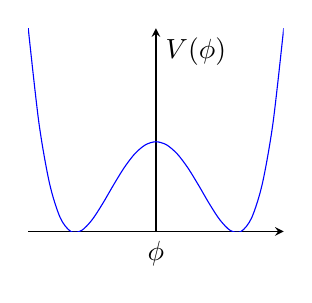
\begin{tikzpicture}
\begin{axis}[width=1.9in,axis x line=middle, axis y line=center, 
			ticks=none, xlabel= $\phi$, ylabel = $V(\phi)$,
			xlabel near ticks,
			]
\addplot+[mark=none,smooth] (\x,{(\x^2 - 10)^2});
\end{axis}
\end{tikzpicture}
\caption{The potential described in \autoref{eq:single_real_field_potential}, as a function of a spatially constant field $\phi$.}
\label{fig:single_real_field}
\end{marginfigure}

This Lagrangian is invariant under the reflection of the field, $\phi\rightarrow -\phi$. The Hamiltonian (density) $\mathcal{H}$ can be obtained by performing a Legendre transformation on the Lagrangian:
\begin{align}
\mathcal{H} = \frac{\partial\mathcal{L}}{\partial\dot{\phi}}\dot{\phi} - \mathcal{L} = \frac{1}{2}(\partial_0\phi)^2+ \frac{1}{2}(\nabla\phi)^2+ V(\phi)
\end{align}

The Hamiltonian $\mathcal{H}$ corresponds to an energy density, with the kinetic energy, $\mathcal{K} = \frac{1}{2}(\partial_0\phi)^2$ and the potential energy $\mathcal{V} = \frac{1}{2}(\nabla\phi)^2 + V(\phi)$. Since $(\nabla\phi)^2 \geq 0$ The minimum of this potential energy is achieved when $\nabla\phi = 0$, that is, the field must be a constant in space - let us denote this minimum constant value by $\phi_0$. The two possibilities for $\phi_0$ that minimize the potential in \autoref{fig:single_real_field} are $\phi_0 = \pm\sqrt{m^2/\lambda}$. The ground state of the theory must correspond to one of these.

Since it does not matter which minimum we choose, we can arbitrarily choose the positive value. This is known as the the \emph{vacuum expectation value} (\textsc{vev}). Having chosen this minimum, we can rewrite our Lagrangian in terms of the field $\phi' = \phi - \sqrt{m^2/\lambda}$ (note that we can do this because the physics remains the same under this translational redefinition of the field):
\begin{marginfigure}
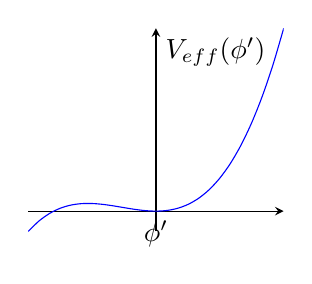
\begin{tikzpicture}
\begin{axis}[width=1.9in,axis x line=middle, axis y line=center, 
			ticks=none, xlabel= $\phi'$, ylabel = $V_\text{eff}(\phi')$,
			xlabel near ticks,
			]
\addplot+[mark=none,smooth] (\x,{10*\x^3 + 40*\x^2});
\end{axis}
\end{tikzpicture}
\caption{The potential (\autoref{eq:potential_hidden_symmetry}) `seen' by the ground state, as a function of a spatially constant field $\phi'$.}
\label{fig:hidden_symmetry}
\end{marginfigure}

\begin{align}
\mathcal{L}(\phi') = \frac{1}{2}\partial^\mu\phi'\partial_\mu\phi' - V_\text{eff}(\phi')\\
V_\text{eff}(\phi') = \frac{\lambda}{4} + \sqrt{\frac{m^2}{\lambda}}\phi'^3 + m^2\phi'^2
\label{eq:potential_hidden_symmetry}
\end{align}
This Lagrangian is no longer symmetric under reflection, i.e. it is not invariant under the transformation $\phi'\rightarrow -\phi'$. This potential is minimized at $\phi' = 0$, which is convenient for performing perturbation theory. The mass of physical particles corresponding to quantum fluctuations of this vacuum is given by $V''_\text{eff}\|_{\phi' = 0} = \sqrt{2}m$. Note that we have not done anything to the system to break this symmetry. The symmetry of the original Lagrangian is hidden in the relationships between the coefficients of the terms of the new Lagrangian. Keeping the above in mind, it might be more helpful to think about the symmetry as being \emph{hidden} by choosing a particular \textsc{vev}.

\subsection{Single complex field}

What if the field $\phi$ was complex, instead of real? It would then have an additional degree of freedom, contributed by its imaginary component. This makes it possible for the Lagrangian to have a continuous symmetry, as opposed to the discrete reflection symmetry in the previous example. The potential has the same general structure:
\begin{align}
V(\phi) = \frac{\lambda}{4}\left(\phi^{*}\phi - \frac{m^2}{\lambda}\right)^2
\label{eq:single_complex_field_potential}
\end{align}

\begin{marginfigure}
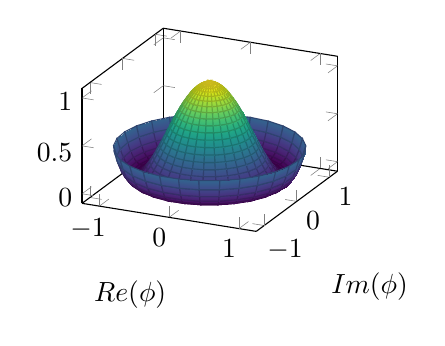
\begin{tikzpicture}
\begin{axis}[
			xlabel=$Re(\phi)$,
			ylabel=$Im(\phi)$,
			% zlabel=$V(\phi)$,
			colormap name = viridis,
			width=1.9in,
            samples=30,
            domain=0:360,
            y domain=0:1.25,
        ]
        \addplot3 [surf, 
					shader=faceted interp,
				ticks=none,
				   z buffer=sort] ({sin(x)*y}, {cos(x)*y}, {(y^2-1)^2});
        \end{axis}
\end{tikzpicture}
\caption{The infamous `Mexican hat potential.The masses of the fields depend upon where the theory 'lives'. }.
\end{marginfigure}

In this case, the Lagrangian has an additional symmetry, known as
global U(1) symmetry. This means that it is invariant under transfor- mations of the form $\phi\rightarrow e^{i\theta}\phi$ where $\theta$ is a parameter independent of space-time. The form of transformation suggests rotations, and indeed we can see that this potential will be invariant under rotations about its symmetry axis \footnote{ The reflection symmetry from the previous example is incorporated here - it is nothing but a U(1) transformation with $\theta = \pi$.}.

We can pick any of the points at the minimum of this potential as a vacuum expectation value. To recover a similar scenario as the previous example, we can pick $\phi_0 = \sqrt{m^2/\lambda}$. This reproduces a theory with a particle of mass $\sqrt{2}m$.

You can imagine the potential as a surface along which a ball rolls, and the the mass to be analogous to the `resistance' the ball faces from the surface it if tries to roll. This resistance is given by the curvature of the surface - the second derivative of the potential function.
At $\phi = 0$ there is `negative resistance', corresponding to tachyons with imaginary mass, whereas if it resides in one of the troughs, then it would face some resistance, corresponding to particles with positive mass.

We see that the curvature in the radial direction will provide some resistance, but there is no curvature in the angular direction - the ball can roll around in a circle without any resistance. Since the curvature in the angular direction is zero, the mass of the particle will be zero.

Basically, we can write our single complex field in terms of two real fields, one corresponding to the radial degree of freedom and the other corresponding to the angular degree of freedom. We can interpret these two real fields as particles. The field that can only change in the radial direction now has positive mass, whereas the field that can change in the angular direction is massless. This field corresponds to a massless particle, termed the Goldstone boson.

In fact, this is but an example of a more general result known as \emph{Goldstone's theorem}, which states that for every spontaneous breaking of a continuous symmetry, there appears a set of massless scalar bosons corresponding to the generators of the symmetry group.

\subsection{Local U(1) symmetry}

We have already seen in \autoref{sec:gauge_invariance} an example of the ramifications of an unbroken $U(1)$ gauge symmetry, which led to a structure very much like QED, with massless photons. Let us now see what happens when this symmetry is spontaneously broken. Our Lagrangian is the same as that for previous example with a single complex field, but now invariant under transformations of the form $\phi\rightarrow e^{i\theta(x)}$, where $\theta(x)$ is now a function of space and time.  Like before, we promote the partial derivatives $\partial_\mu$ to covariant derivatives $\partial_\mu - igA_\mu$, where the vector field $A_\mu$ transforms as $A_\mu + \frac{1}{g}\partial_\mu\theta(x)$. Our Lagrangian now reads
\begin{align}
\mathcal{L}(\phi) &= \frac{1}{2} D^\mu\phi D_\mu\phi - V(\phi)-\frac{1}{4}F_{\mu\nu}F^{\mu\nu}\\
V(\phi) &= \lambda\left(\phi^*\phi - \frac{v^2}{2}\right)^2
\end{align}
where $V(\phi)$ is the same as in \autoref{eq:single_complex_field_potential}.

We can now proceed with spontaneously breaking this symmetry. To do so, we choose a vacuum expectation value $\langle\phi\rangle = v/\sqrt{2}$ We can write our original complex field as $\phi = e^{i\xi/v}(v+\rho)/2$, where $\xi$ and $\rho$ are two real fields corresponding to the angular and radial degrees of freedom respectively. When we pick the vacuum expectation value $v/\sqrt{2}$, this sets $\langle\xi\rangle = \langle\rho\rangle=0$. We can then write the Lagrangian in terms of $\xi$ and $\rho$ as follows:
\begin{equation*}
\mathcal{L}(\xi,\rho) = \frac{1}{2}\partial_\mu\rho\partial^\mu\rho + \frac{(v + \rho)^2}{2}%
\left(-gA_\mu+\frac{\partial_\mu\xi}{v}\right)^2-\frac{\lambda}{4}\left(\rho^2 + 2v\rho^2\right)^2%
-\frac{1}{4}F_{\mu\nu}F^{\mu\nu}
\end{equation*}
In this form, we see that there is a mass term of the form $A_\mu A^\mu$ for the gauge field. However, there is also a mixed term, $-gvA_\mu\partial^\mu\xi$ whose interpretation is not immediately clear. We can fix this by choosing a gauge that makes $\phi$ always real:
$\theta(x) = \frac{\xi(x)}{gv}$
When we do so, the terms with $\xi$ disappear. Thus, gathering the terms in the Lagrangian quadratic in the fields, we get
\begin{equation}
\mathcal{L}_\text{quadratic}^\text{unitary gauge} = \frac{1}{2}\partial_\mu\rho\partial^\mu\rho + g^2v^2 A_\mu A^\mu - \lambda v^2\rho^2 - \frac{1}{4}F_{\mu\nu}F^{\mu\nu}
\end{equation}
We see that the field $A_\mu$ acquires a mass of $gv$ and the field that changes along the radial direction, $\rho$, acquires a mass as well. We term this field the physical \emph{Higgs boson}. We seem to have gotten rid of the Goldstone boson that should appear due to Goldstone’s theorem! However, upon closer inspection, we see that the Goldstone boson is just hidden in the theory as an extra degree of freedom. After symmetry breaking, the massless gauge field combines with one of the scalar fields to form a massive vector field. We can shed some light on the situation by examining the degrees of freedom. The gauge field originally had two degrees of freedom corresponding
to the two possible polarization states, and the $\xi$ and $\rho$ had one degree of freedom each. The $\rho$ retained its degree of freedom, but the vector boson field now has three degrees of freedom (three possible polarization states) after `eating' the $\xi$ field. The $\xi$ field is called a `would-be' Goldstone boson. We have just finished describing the Higgs mechanism for the spontaneous breaking of an Abelian symmetry.

\section{Electroweak symmetry breaking}

Now, instead of a single complex field, let us consider a field $H$ that transforms as a doublet under $SU(2)$ transformations. We can write $H$ as:
$$H = \begin{pmatrix}H^{+}\\H^0\end{pmatrix}$$
The terms of the Lagrangian that involve this field can be written as follows:
\begin{align*}
  \mathcal{L}_{\text{Higgs}} &= \frac{1}{2}\left|D_\mu H\right|^2-V(H)\\
  V(H) &= \left(H^\dag H-\frac{v^2}{2}\right)^2
\end{align*}
This Lagrangian is invariant under $U(1)$ transformations. It is also invariant under $SU(2)$ transformations of the form $H\rightarrow e^{i\epsilon_a(x)T^a}H$. Here, $\epsilon_a (x)$ is a space-time dependent parameter and $T_a = \sfrac{\tau_a}{2}$, where $\tau_a$ are the familiar Pauli matrices.

Since we have three generators $(T_a)$ for the $SU(2)$ symmetries, and one $(Y)$ for the $U(1)$ symmetry, we will introduce four gauge fields to construct the covariant derivative $D_\mu$.
\begin{align*}
  SU(2)&\rightarrow W_\mu^1,W_\mu^2, W_\mu^3\\
  U(1)&\rightarrow B_\mu
\end{align*}
Thus the gauge covariant derivative takes the form
$$D_\mu = \partial_\mu + igW_\mu^a\frac{\tau^a}{2}+ig'YB_\mu.$$
The potential $V(H)$ reaches its minimum when $H^\dag H = v^2 / 2$. We can pick a vacuum expectation value for $H$ that breaks the neutral sector symmetry (corresponding to $H^0$) but not the charged symmetry (corresponding to $H^{+}$), since we know that electromagnetic gauge invariance is a good symmetry to keep, because photons are massless. Thus, we can write the doublet field as
$$H = \left(\begin{array}{c}0\\\frac{v}{\sqrt{2}}\end{array}\right).$$
We combine $W_\mu^1$ and $W_\mu^2$ to form two composite fields, $W^\pm$, as follows.
$$W_\mu^\pm = \frac{W_\mu^1\pm iW_\mu^2}{\sqrt{2}}$$
We use this redefinition and plug in our value for the vacuum expectation value into the kinetic term of the Lagrangian.
\begin{align*}
  (D_\mu H)^\dag(D_\mu H) &= (\begin{array}{cc} 0 & \frac{v}{\sqrt{2}}\end{array})
  \left(\partial_\mu - igW_\mu^a\frac{\tau^a}{2}
  -\frac{ig'}{2}B_\mu\right)
  \left(\partial_\mu+igW_\mu^a\frac{\tau^a}{2}+\frac{ig'}{2}B_\mu\right)
  \left(\begin{array}{c}0\\\frac{v}{\sqrt{2}}\end{array}\right)\\
  W_\mu^a\frac{\tau^a}{2} &= 
  \frac{1}{\sqrt{2}}
  \left(\begin{array}{cc}
    \frac{W_\mu^3}{\sqrt{2}} & W_\mu^+\\
    W_\mu^- & -\frac{W_\mu^3}{\sqrt{2}}
  \end{array}\right).
\end{align*}
If we simplify the above expression and isolate the mass terms, we get
\[\frac{g^2v^2}{4}W_\mu^-W_\mu^++\frac{1}{2}\frac{v^2}{4}(g^2+g'^2)
\left(\frac{gW_\mu^3}{\sqrt{g^2+g'^2}}-\frac{g'B_\mu}{\sqrt{g^2+g'^2}}\right)^2\]
We can make the following definitions:
\begin{align*}
  \frac{g}{\sqrt{g^2+g'^2}} = \cos\theta &&
  \frac{g'}{\sqrt{g^2+g'^2}} = \sin\theta
\end{align*}
We also make composite fields out of $W_\mu^3$ and $B_\mu$, namely the Z boson ($Z_\mu$) and the photon ($A_\mu$), with $Z_\mu$ defined as follows.
\[Z_\mu = \frac{gW_\mu^3}{\sqrt{g^2+g'^2}}-\frac{g'B_\mu^3}{\sqrt{g^2+g'^2}}\]
The product $W_\mu^+W_\mu^-$ can be written as a mass term for a generic charged vector boson $W_\mu^\pm$. Rewriting our mass terms for the vector boson fields with the above redefinitions, we get
\[\mathcal{L}_{\text{mass term}}=\frac{e^2v^2}{4\sin^2\theta}W_\mu W^\mu+
\frac{e^2v^2}{8\sin^2\theta\cos^2\theta}Z_\mu Z^\mu\]
After accounting for symmetry factors, we get the masses of the W and Z bosons as:
\begin{align*}
  m_W &=\frac{ev}{2\sin\theta} & 
  m_Z &=\frac{ev}{\sin2\theta}
\end{align*}
We see that there is no mass term for $A_\mu$, which means that this gauge field remains massless. Thus we see that the W and Z bosons gain mass, limiting their range, while the photon remains massless, corresponding to what is experimentally observed. To find out how these gauge particles interact with spin-$\slantfrac{1}{2}$ fermions, we will take the familiar Lagrangian that leads to the Dirac equation:

\section{Interactions}

We have already constructed a gauge-covariant derivative 
$$D_\mu = \partial_\mu + igW_\mu^a T^a + ig'YB_\mu$$
We can write our Lagrangian as
$$i\overline{\psi}_L\gamma^\mu D_\mu\psi_L + i\overline{e_R}\gamma^\mu D_\mu e_R$$
Here, $\psi_L$ is the lepton doublet
$$\begin{pmatrix}\nu_L\\e_L\end{pmatrix}$$
while $e_R$ is a lepton singlet. We do not include $\nu_R$ because there has been no evidence of right-handed neutrinos \footnote{Although we do know now that neutrinos have mass, and the existence of a as-yet heavy undetected right-handed neutrino is a possible mechanism for generating neutrino masses}. The left- and right-handed fields are obtained by having the projection operators $P_L$ and $P_R$ on the lepton field. The $SU(2)$ transformation only acts on the left-handed field, while the $U(1)$ transformation acts on both the left- and right-handed fields. We will first derive the interactions for the left-handed field, and then consider the right-handed field. The charges of the different components of the doublet under different symmetry groups is given in \autoref{tab:charges}
\begin{margintable}
  \centering
  \begin{tabular}{rlll}
    Field & $T_3$ & $Y$ & $Q$ \\
  \hline
  $\nu_L$ & $\slantfrac{1}{2}$ & $-\slantfrac{1}{2}$ & 0\\
  $e_L$ & $-\slantfrac{1}{2}$ & $-\slantfrac{1}{2}$ & 1\\
  \end{tabular}
  \caption{Charges of the various fields}
  \label{tab:charges}
\end{margintable}
\begin{equation}
  \mathcal{L}_\text{interaction terms} = -\frac{g}{\sqrt{2}}
  \begin{pmatrix}
    \bar{\nu_L} & \bar{e_L}
  \end{pmatrix}
  \gamma^\mu
  \begin{pmatrix}
    \frac{W_\mu^3}{\sqrt{2}} & W_\mu^+\\
    W_\mu^- & -\frac{W_\mu^3}{\sqrt{2}}
  \end{pmatrix}
  \begin{pmatrix}
    \nu_L \\ e_L
  \end{pmatrix}
  -g'Y
  \begin{pmatrix}
    \bar{\nu_L} & \bar{e_L}
  \end{pmatrix}
  \gamma^\mu
  \begin{pmatrix}
    \nu_L \\ e_L
  \end{pmatrix}
\end{equation}
\subsection{Charged sector}
We will first consider the charged fields $W^\pm$. To do this, we will isolate the terms in the covariant derivative $D_\mu$ that correspond to them, that is, the terms containing $W_1^\mu$ and $W_\mu^2$. Writing this out, we get:
$$-\frac{g}{\sqrt{2}}\bar{\nu_L}\gamma^\mu W_\mu^+ e_L - \frac{g}{\sqrt{2}}\bar{e_L}\gamma^\mu W_\mu^- \nu_L$$
These give us Feynman diagram vertices for the interactions mediated by W bosons.
\subsection{Neutral sector}
We can apply a similar treatment to the neutral gauge particles $A_\mu$ and $Z_\mu$. Isolating the coupling terms in the covariant derivative, we get
\[gW_\mu^3T_3 + g'B_\mu Y\]
Remembering our previous definitions of $g$ and $g'$ in terms of the mixing angle $\theta$, we can write the expressions for $Z_\mu$ and its orthogonal field $A_\mu$.
\newcommand{\ct}{\cos\theta}
\newcommand{\st}{\sin\theta}
$$
\fourmatrix{\ct}{-\st}{\st}{\ct}
\vdoublet{W_{\mu}^{3}}{B_{\mu}} =  \vdoublet{Z_\mu}{A_\mu}
$$
We can invert this matrix to find $Z_\mu$ and $A_\mu$ in terms of $W_\mu^3$ and $B_\mu$. Doing so, we get
$$\vdoublet{W_\mu^3}{B_\mu} = \fourmatrix{\cos\theta}{-\sin\theta}{\sin\theta}{\cos\theta}\vdoublet{W_{\mu}^{3}}{B_{\mu}} =  \vdoublet{Z_\mu}{A_\mu}$$
So we get our coupling terms (which will be flanked on either side by fermion fields, which we have omitted for ease of reading) in the following form:
$$
g(Z_\mu\ct+A_\mu\st)T_3 + g'(-Z_\mu\st+A_\mu\ct)Y\\
= A_\mu(g\st T_3 + g'\ct Y) + Z_\mu(g\ct T_3 - g'\st Y)
$$
But we know that $$g\st = g'\ct = \frac{gg'}{\sqrt{g^2 + g'^2}}.$$
So our photon coupling then becomes 
$$A_\mu\left(\frac{gg'}{\sqrt{g^2 + g'^2}}\right)(T_3 + Y)$$
We know that the strength of the electromagnetic interaction depends on the magnitude of the electric charge. Keeping this in mind, we relabel the constant $gg'/\sqrt{g^2 + g'^2}$ as $e$, and the operator $T_3 + Y$ as $Q$, the charge matrix. Thus the electron will have a charge of $-e$ and the up quark will have a charge of $\slantfrac{2}{3} e$, and so on. So now we have $g$ and $g'$ in terms of $\theta$ and $e$, and we can substitute those definitions into the $Z$ coupling to get:
$$Z_\mu\frac{e}{\st\ct}(T_3 - \sin^2\theta Q)$$

For the quarks, the flavor and mass eigenstates are related by the Cabibbo-Kobayashi-Maskawa mixing matrix:

\begin{equation}
  V_\text{CKM} =
  \begin{pmatrix}
    V_{ud} & V_{us} & V_{ub}\\
    V_{cd} & V_{cs} & V_{cb}\\
    V_{td} & V_{ts} & V_{tb}
  \end{pmatrix}
\end{equation}

\section{Limits of the Standard Model}
By now we have reached the frontier of particle physics. The community is 

We still don't know what dark matter is

Why does the Higgs have the mass it does? (Hierarchy problem)

Neutrino masses?
